
\begin{centering}
\bf Laboratorio de M\'etodos Num\'ericos - Segundo Cuatrimestre 2015 \\
\bf Trabajo Pr\'actico N\'umero 1: Con 15 $\theta$s discretizo alto horno\ldots\\
\end{centering}

\vskip 25pt
\hrule
\vskip 11pt

{\bf Introducción}

Consideremos la secci\'on horizontal de un horno de acero cil\'indrico, como en la Figura 1. El sector A es la pared del horno, y el sector B es el horno propiamente dicho, en el cual se funde el acero a temperaturas elevadas. Tanto el borde externo como el borde interno de la pared forman c\'irculos. Suponemos que la temperatura del acero dentro del horno (o sea, dentro de B) es constante e igual a 1500$^{o}$C.

\medskip

Tenemos sensores ubicados en la parte externa del horno para medir la temperatura de la pared externa del mismo, que habitualmente se encuentra entre 50$^{o}$C y 200$^{o}$C. El problema que debemos resolver consiste en estimar la isoterma de 500$^{o}$C dentro de la pared del horno, para estimar la resistencia de la misma. Si esta isoterma est\'a demasiado cerca de la pared externa del horno, existe peligro de que la estructura externa de la pared colapse.


\begin{figure}[ht]
\begin{center}
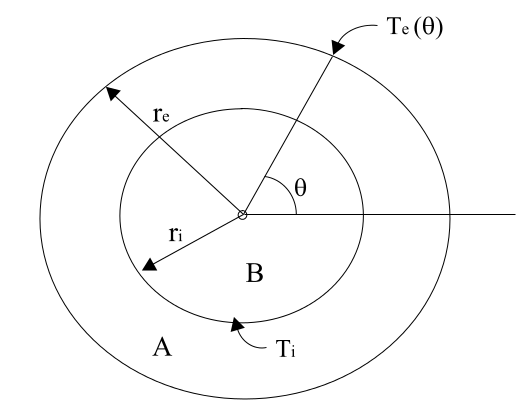
\includegraphics[width=0.6\columnwidth]{img/Horno.png}
\caption{Secci\'on circular del horno}
\end{center}
\end{figure}



El objetivo del trabajo práctico es implementar un programa que calcule la isoterma solicitada, conociendo las dimensiones del horno y las mediciones de temperatura en la pared exterior.

{\bf El Modelo}

Sea $r_e \in \mathbb{R}$ el radio exterior de la pared y sea $r_i \in \mathbb{R}$ el radio interior de la pared. Llamemos $T(r,\theta)$ a la temperatura en el punto dado por las coordenadas polares $(r,\theta)$, siendo $r$ el radio y $\theta$ el \'angulo polar de dicho punto. En el estado estacionario, esta temperatura satisface la ecuaci\'on del calor:

\begin{equation}\label{calor}
\frac{\partial^2T(r,\theta)}{\partial r^2}+\frac{1}{r}\frac{\partial T(r,\theta)}{\partial r}+\frac{1}{r^2}\frac{\partial^2T(r,\theta)}{\partial \theta^2} = 0 
\end{equation}


Si llamamos $T_i \in \mathbb{R}$ a la temperatura en el interior del horno (sector B) y $T_e : [0,2\pi] \rightarrow \mathbb{R}$ a la funci\'on de temperatura en el borde exterior del horno (de modo tal que el punto $(r_e,\theta)$ tiene temperatura $T_e(\theta)$), entonces tenemos que

\begin{equation}
T(r,\theta) = T_i \;\;\;\;\;para\;todo\;punto\;(r,\theta)\;con\;r\leq r_i
\end{equation}
\begin{equation}
T(r_e,\theta) = T_e(\theta) \;\;\;\;\;\;para\;todo\;punto\;(r_e,\theta)
\end{equation}


El problema en derivadas parciales dado por la primera ecuaci\'on con las condiciones de contorno presentadas recientemente, permite encontrar la funci\'on $T$ de temperatura en el interior del horno (sector A), en funci\'on de los datos mencionados en esta secci\'on.

Para resolver este problema computacionalmente, discretizamos el dominio del problema (el sector A) en coordenadas polares. Consideramos una partici\'on $0 = \theta_0 < \theta_1 < ... < \theta_n = 2\pi$ en $n$ \'angulos discretos con $\theta_k-\theta_{k-1} = \Delta\theta$ para $k = 1,...,n$, y una partici\'on $r_i = r_0 < r_1 < ... < r_m = r_e$ en $m+1$ radios discretos con $r_j - r_{j-1} = \Delta r$ para $j = 1,...,m$.

\medskip

El problema ahora consiste en determinar el valor de la funci\'on $T$ en los puntos de la discretizaci\'on $(r_j,\theta_k)$ que se encuentren dentro del sector A. Llamemos $t_{jk} = T(r_j,\theta_k)$ al valor (desconocido) de la funci\'on $T$ en el punto $(r_j,\theta_k)$.

\medskip

Para encontrar estos valores, transformamos la ecuaci\'on (\ref{calor}) en un conjunto de ecuaciones lineales sobre las inc\'ognitas $t_{jk}$, evaluando (\ref{calor}) en todos los puntos de la discretizaci\'on que se encuentren dentro del sector A. Al hacer esta evaluaci\'on, aproximamos las derivadas parciales de $T$ en (\ref{calor}) por medio de las siguientes f\'ormulas de diferencias finitas:


\begin{equation}
\frac{\partial^2T(r,\theta)}{\partial r^2}(r_j,\theta_k) \cong \frac{t_{j-1,k}-2t_{jk}+t_{j+1,k}}{(\Delta r)^2}
\end{equation}

\begin{equation}
\frac{\partial T(r,\theta)}{\partial r}(r_j,\theta_k) \cong \frac{t_{j,k}-t_{j-1,k}}{\Delta r}
\end{equation}

\begin{equation}
\frac{\partial^2T(r,\theta)}{\partial \theta^2}(r_j,\theta_k) \cong \frac{t_{j,k-1}-2t_{jk}+t_{j,k+1}}{(\Delta \theta)^2}
\end{equation}



Es importante notar que los valores de las inc\'ognitas son conocidos para los puntos que se encuentran sobre el borde exterior de la pared, y para los puntos que se encuentren dentro del sector B. Al realizar este procedimiento, obtenemos un sistema de ecuaciones lineales que modela el problema discretizado. La resoluci\'on de este sistema permite obtener una aproximaci\'on de los valores de la funci\'on $T$ en los puntos de la discretizaci\'on.

{\bf Enunciado}

Se debe implementar un programa en \verb+C+ o \verb-C++- que tome como entrada los par\'ametros del problema ($r_i$, $r_e$, $m+1$,
$n$, valor de la isoterma buscada, $T_i$, $T_e(\theta)$) que calcule la temperatura dentro de la pared del horno utilizando el
modelo propuesto en la secci\'on anterior y que encuentre la isoterma buscada en funci\'on del resultado obtenido del
sistema de ecuaciones. El m\'etodo para determinar la posici\'on de la isoterma queda a libre elecci\'on de cada grupo y
debe ser explicado en detalle en el informe.

El programa debe formular el sistema obtenido a partir de las ecuaciones (1) - (6) y considerar dos m\'etodos posibles
para su resoluci\'on: mediante el algoritmo cl\'asico de Eliminaci\'on Gaussiana y la Factorizaci\'on LU. Finalmente, el
programa escribir\'a en un archivo la soluci\'on obtenida con el formato especificado en la siguiente secci\'on.

Como ya se ha visto en la materia, no es posible aplicar los m\'etodos propuestos para la resoluci\'on a cualquier
sistema de ecuaciones. Sin embargo, la matriz del sistema considerado en el presente trabajo cumple con ser diagonal dominante (no
estricto) y que, ordenando las variables y ecuaciones convenientemente, es posible armar un sistema de ecuaciones cuya matriz
posee la propiedad de ser \emph{banda}. Luego, se pide demostrar (o al menos dar un esquema de la demostraci\'on)
el siguiente resultado e incluirlo en el informe:

\begin{proposition}
Sea $A \in \mathbb{R}^{n \times n}$ la matriz obtenida para el sistema definido por (1)-(6). Demostrar que es posible
aplicar Eliminaci\'on Gaussiana sin pivoteo.\footnote{Sugerencia: Notar que la matriz es diagonal dominante (no
estrictamente) y analizar qué sucede al aplicar un paso de Eliminaci\'on Gaussiana con los elementos de una fila.} 
\end{proposition}

La soluci\'on del sistema de ecuaciones permitir\'a saber la temperatura en los puntos de la discretizaci\'on. Sin embargo,
nuestro inter\'es es calcular la isoterma 500, para poder determinar si la estructura se encuentra en peligro. Luego, se pide lo siguiente:
\begin{itemize}
\item Dada la soluci\'on del sistema de ecuaciones, proponer una forma de estimar en cada \'angulo de la discretizaci\'on la posici\'on de la 
isoterma 500.
\item En funci\'on de la aproximaci\'on de la isoterma, proponer una forma (o medida) a utilizar para evaluar la peligrosidad de la estructura
en funci\'on de la distancia a la pared externa del horno.
\end{itemize}


En funci\'on de la experimentaci\'on, se busca realizar dos estudios complementarios: por un lado, analizar c\'omo se comporta el sistema y, por otro, 
cu\'ales son los requerimientos computacionales de los m\'etodos. Se pide como m\'inimo realizar los siguientes experimentos:
\begin{enumerate}
\item Comportamiento del sistema.
\begin{itemize}
\item Considerar al menos dos instancias de prueba, generando distintas discretizaciones para cada una de ellas y
comparando la ubicaci\'on de la isoterma buscada respecto de la pared externa del horno. Se sugiere presentar gr\'aficos
de temperatura o curvas de nivel para los mismos, ya sea utilizando las herramientas provistas por la c\'atedra o
implementando sus propias herramientas de graficaci\'on. 
\item Estudiar la proximidad de la isoterma buscada respecto de la pared exterior del horno en funci\'on de distintas 
granularidades de discretizaci\'on y las condiciones de borde. 
\end{itemize}
\item Evaluaci\'on de los m\'etodos.
\begin{itemize}
\item Analizar el tiempo de c\'omputo requerido para obtener la soluci\'on del sistema en funci\'on de la granularidad de 
la discretizaci\'on. Se sugiere presentar los resultados mediante gr\'aficos de tiempo de c\'omputo en funci\'on de alguna 
de las variables del problema.
\item Considerar un escenario similar al propuesto en el experimento 1. pero donde las condiciones de borde (i.e., $T_i$ y $T_e(\theta)$)
cambian en distintos instantes de tiempo. En este caso, buscamos obtener la secuencia de estados de la temperatura en
la pared del horno, y la respectiva ubicaci\'on de la isoterma especificada. Para ello, se considera una secuencia de $ninst$
vectores con las condiciones de borde, y las temperaturas en cada estado es la soluci\'on del correspondiente sistema de
ecuaciones. Se pide formular al menos un experimento de este tipo, aplicar los m\'etodos de resoluci\'on propuestos de
forma conveniente y compararlos en t\'erminos de tiempo total de c\'omputo requerido para distintos valores de $ninst$.
\end{itemize}
\end{enumerate}

De manera opcional, aquellos grupos que quieran ir un poco m\'as all\'a pueden considerar trabajar y desarrollar alguno(s) 
de los siguientes puntos extra:
\begin{enumerate}
\item Notar que el sistema resultante tiene estructura \emph{banda}. Proponer una estructura para aprovechar este hecho en t\'erminos de la
\emph{complejidad espacial} y como se adaptar\'ian los algoritmos de Eliminaci\'on Gaussiana y Factorizaci\'on LU para reducir la
cantidad de operaciones a realizar.
\item Implementar dicha estructura y las adaptaciones necesarias para el algoritmo de Eliminaci\'on Gaussiana.
\item Implementar dicha estructura y las adaptaciones necesarias para el algoritmo de Factorizaci\'on LU. 
\end{enumerate}

Finalmente, se deber\'a presentar un informe que incluya una descripci\'on detallada de los m\'etodos implementados y
las decisiones tomadas, el m\'etodo propuesto para el c\'alculo de la isoterma buscada y los experimentos realizados,
junto con el correspondiente an\'alisis y siguiendo las pautas definidas en el archivo \verb+pautas.pdf+.

{\bf Programa y formato de archivos}

Se deber\'an entregar los archivos fuentes que contengan la resoluci\'on del trabajo pr\'actico. El ejecutable tomar\'a
tres par\'ametros por l\'inea de comando, que ser\'an el archivo de entrada, el archivo de salida, y el m\'etodo a
ejectutar (0 EG, 1 LU).

El archivo de entrada tendr\'a la siguiente estructura:
\begin{itemize}
\item La primera l\'inea contendr\'a los valores $r_i$, $r_e$, $m+1$, $n$, $iso$, $ninst$, donde $iso$ representa el
valor de la isoterma buscada y $ninst$ es la cantidad de instancias del problema a resolver para los par\'ametros dados.
\item A continuaci\'on, el archivo contendr\'a $ninst$ l\'ineas, cada una de ellas con $2n$ valores, los primeros $n$ indicando los
valores de la temperatura en la pared interna, i.e., $T_i(\theta_0),T_i(\theta_1),\dots,T_i(\theta_{n-1})$, seguidos de $n$ valores
de la temperatura en la pared externa, i.e., $T_e(\theta_0)$,$T_e(\theta_1)$,$\dots$,$T_e(\theta_{n-1})$.
\end{itemize}

El archivo de salida obligatorio tendr\'a el vector soluci\'on del sistema reportando una componente del mismo por
l\'inea. En caso de $ninst > 1$, los vectores ser\'an reportados uno debajo del otro.

Junto con el presente enunciado, se adjunta una serie de scripts hechos en \verb+python+ y un conjunto instancias de
test que deber\'an ser utilizados para la compilaci\'on y un testeo b\'asico de la implementaci\'on. Se recomienda leer
el archivo \verb+README.txt+ con el detalle sobre su utilizaci\'on.

{\bf \underline{Fechas de entrega}}
\begin{itemize}
\item \emph{Formato Electr\'onico:} Jueves 3 de Septiembre de 2015, hasta las 23:59 hs, enviando el trabajo (informe +
c\'odigo) a la direcci\'on \verb+metnum.lab@gmail.com+. El subject del email debe comenzar con el texto \verb+[TP1]+
seguido de la lista de apellidos de los integrantes del grupo.
\item \emph{Formato f\'isico:} Viernes 4 de Septiembre de 2015, de 17:30 a 18:00 hs.
\end{itemize}

\noindent \textbf{Importante:} El horario es estricto. Los correos recibidos despu\'es de la hora indicada ser\'an
considerados re-entrega. Los grupos deben ser de 3 o 4 personas, sin excepci\'on. Es indispensable que los trabajos
pasen satisfactoriamente los casos de test provistos por la c\'atedra.
